%!TEX program = xelatex
\documentclass[14pt]{scrartcl} % A4 paper and 11pt font size
\usepackage[UTF8]{ctex}
\usepackage{lmodern}
\usepackage{amsmath}
\usepackage{amsfonts}
\usepackage{amssymb}
\usepackage[T1]{fontenc} % Use 8-bit encoding that has 256 glyphs
\usepackage{fourier} % Use the Adobe Utopia font for the document - comment this line to return to the LaTeX default
\usepackage[english]{babel} % English language/hyphenation
\usepackage{amsmath,amsfonts,amsthm} % Math packages
\usepackage{graphicx}
\usepackage{epstopdf}
\epstopdfsetup{outdir=./}
\usepackage{float}
\usepackage{lipsum} % Used for inserting dummy 'Lorem ipsum' text into the template
\usepackage{enumerate}
\usepackage{fancyvrb}
\usepackage{sectsty} % Allows customizing section commands
\allsectionsfont{\centering \normalfont\scshape} % Make all sections centered, the default font and small caps



\numberwithin{equation}{section} % Number equations within sections (i.e. 1.1, 1.2, 2.1, 2.2 instead of 1, 2, 3, 4)
\numberwithin{figure}{section} % Number figures within sections (i.e. 1.1, 1.2, 2.1, 2.2 instead of 1, 2, 3, 4)
\numberwithin{table}{section} % Number tables within sections (i.e. 1.1, 1.2, 2.1, 2.2 instead of 1, 2, 3, 4)

\setlength\parindent{0pt} % Removes all indentation from paragraphs - comment this line for an assignment with lots of text

%----------------------------------------------------------------------------------------
%	TITLE SECTION
%----------------------------------------------------------------------------------------

\newcommand{\horrule}[1]{\rule{\linewidth}{#1}} % Create horizontal rule command with 1 argument of height
\newcommand*{\Scale}[2][4]{\scalebox{#1}{$#2$}}%
\title{	
	\normalfont \huge
	\textsc{概率统计} \\ [25pt] % Your university, school and/or department name(s)
	\horrule{0.5pt} \\[0.4cm] % Thin top horizontal rule
	\huge 第二周作业答案 \\ % The assignment title
	\horrule{0.5pt} \\[0.4cm] % Thick bottom horizontal rule
	\date{}
}

\begin{document}
	\maketitle % Print the title
	15.已知 $P(A)=\frac{1}{4}, P(B \mid A)=\frac{1}{3}, P(A \mid B)=\frac{1}{2}$, 求 $P(\bar{A} \bar{B})$ 
	
	\vspace*{1cm}
	\[
	P(B) = \frac{P(A \cap B)}{P(A | B)} = \frac{P(A) P(B | A)}{P(A | B)} = \frac{1 / 4 \times 1 / 3}{1 / 2} = 1 / 6
	\]
	\begin{align}
		P(\bar{A} \cap \bar{B}) & = 1 - P(\overline{\bar{A} \cap \bar{B}}) \\
		& = 1 - P(A \cup B) \\
		& = 1 - (P(A) + P(B) - P(A \cap B)) \\
		& = 1 - (1 / 4 + 1 / 6 - 1 / 4 \times 1 / 3) \\
		& = 1 - 1 / 3 \\
		& = 2 / 3
	\end{align}
	
	\vspace{1cm}
	
	20. 某种元件每盒 20 只, 每盒含 $0,1,2$ 只次品的概率为 $0.8,0.1,0.1$ 。抽样检验, 规定抽检 4 只, 若无次品, 则可出厂。(1) 任取一盒, 求可以出厂的概率; (2) 已知一盒元件可以出厂, 求该盒元件无次品 的概率。
	
	\vspace*{1cm}
	解:$A_i:$盒中有$i$件次品,$i = 1, 2$。$B:$可以出厂。
	\begin{enumerate}[(1)]
		\item
		\begin{align}
			P(B) & = P(A_0)P(B | A_0) + P(A_1)P(B | A_1) + P(A_2)P(B | A_2) \\
			& = 0.8 \times 1 + 0.1 \times \frac{C_{19}^4}{C_{20}^4} + 0.1 \times\frac{C_{18}^4}{C_{20}^4} \\
			& = 0.943
		\end{align}
		\item 
		\[P(A_0 | B) = \frac{P(A_0)P(B | A_0)}{P(B)} = \frac{0.8 \times 1}{0.943} = 0.848\]
	\end{enumerate}
	
	\vspace*{1cm}
	22 . 甲、乙、丙三门炮独立向敌机各射击 1 炮, 设甲、乙、丙的命中率分别为 $0.4,0.5,0.65$ 。敌机中 一炮被击落的概率为 0.4 , 中两炮被击落概率 0.8 , 中三炮必被击落。求敌机被击落概率。
	
	\vspace*{1cm}
	解:$A_1:\text{甲中}, A_2:\text{乙中},A_3:\text{丙中},B:\text{击落}$。
	\begin{align}
		& P(\{\text{中一炮}\}) \\
		& = P((A_1 \cap \bar{A_2} \cap \bar{A_3}) \cup (\bar{A_1} \cap A_2 \cap \bar{A_3}) \cup (\bar{A_1} \cap \bar{A_2} \cap A_3)) \\
		& = P(A_1 \cap \bar{A_2} \cap \bar{A_3}) + P(\bar{A_1} \cap A_2 \cap \bar{A_3}) + P(\bar{A_1} \cap \bar{A_2} \cap A_3)) \\
		& = 0.4 \times 0.5 \times 0.35 + 0.6 \times 0.5 \times 0.35 + 0.6 \times 0.5 \times 065 \\
		& = 0.37
	\end{align}
	同理:
	\begin{align}
		P(\{\text{中两炮}\}) & = 0.6 \times 0.5 \times 0.65 + 0.4 \times 0.5 \times 0.65 + 0.4 \times 0.5 \times 0.35 \\
		& = 0.395
	\end{align}
	$P(\text{中三炮}) = 0.4 \times 0.5 \times 0.65 = 0.13$
	\begin{align}
		& P(B)  \\
		& = P(\{\text{中一炮}\})P(B | \{\text{中一炮}\}) + P(\{\text{中两炮}\})P(B | \{\text{中两炮}\}) + P(\{\text{中三炮}\})P(B | \{\text{中三炮}\}) \\
		& = 0.37 \times 0.4 + 0.395 \times 0.8 + 0.13 \times 1 \\ 
		& = 0.594
	\end{align}
	
	\vspace*{1cm}
	31. 加图 1-19 所示, 系统由 $2 n$ 个独立工作的元件构成, 每个元件的可靠性均为 $p(0<p<1)$ 。试求 该系统的可靠性并且与例 1.25 中的系统比较可靠性大小。
	\begin{figure}[H]
		\centering
		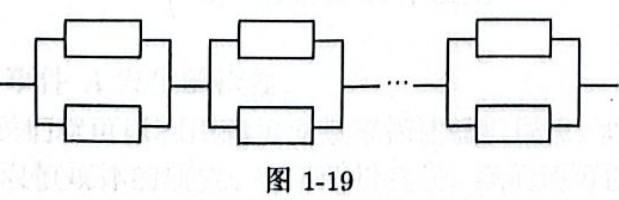
\includegraphics[scale = 0.5]{figures/figure1-19.png}
	\end{figure}
	
	\vspace*{1cm}
	解:每纵列两个元件视为一个子系统。$A_i:$第i个子系统工作,$B:$系统工作。
	易知:$P(A_i) = 1 - (1 - p) ^ 2 = 2p - p ^ 2$, $P_n(B) = P(\cap_{i = 1}^{n} A_i) = (2p - p ^ 2) ^ n = p ^ n ( 2 - p) ^ n$。令$P_n(C) = P(\{\text{例1.25系统工作}\}) = p^n(2 - p ^n)$。
	
	下面只举出两种比较方法:
	
	
	(a)与例1.25系统比较时,假设相同位置使用相同元件,两系统差别只在与连线方式。那么例1.25中系统工作一定可以得出此习题中系统工作。所以习题中系统稳定性大于等于例1.25。
	
	(b) 比较两系统稳定性只需比较$Q_n(B) = (2 - p) ^ n$与$Q_n(C) = 2 - p ^ n$。$n = 1$时$Q_n(B) = Q_n(C)$.$n >1$时
	\begin{align}
		Q_{n + 1}(B) - Q_n(B) & = (2 - p) ^ n(1 - p) \label{eq1}\\
		Q_{n + 1}(C) - Q_n(C) & = p ^ n(1 - p) \label{eq2}
	\end{align}
	(\ref{eq1}) - (\ref{eq2}) = $[(2 - p) ^ n - p ^ n](1 - p)$。因为$p \in(0, 1)$,所以$2 - p > p$,进一步有$(2 - p) ^ n > p ^ n$。可知 (\ref{eq1}) - (\ref{eq2}) > 0。这样$Q_n(B)$增长快于$Q_n(C)$,所以$P_n(B) > P_n(C), \forall n = 2, 3, \dots$
	
\end{document}
